\chapter{Variational Data Assimilation}
\label{var_chap}

An introduction to the basic ideas of variational data assimilation and
the WRF-Var system is given in this chapter, followed by a brief
overview of recent major improvements to WRF-Var.  This overview
supplements the original description of the three-dimensional
variational (3D-Var) algorithm found in \citet{barker04}.  One of the
most important additions to WRF-Var is a new utility {\it gen$\_$be},
used to calculate background error covariances for a user's own
application; it is discussed in the latter half of this chapter.  The
WRF-Var system is evolving rapidly,
and a future technical note will accompany the general release of the
4D-Var component of WRF-Var.  That technical note will include an
extensive description of the entire WRF-Var system.

\section{Introduction}
\label{var-intro}

The basic goal of any variational data assimilation system is to produce
an optimal estimate of the true atmospheric state at analysis time
through iterative solution of a prescribed cost-function \citep{ide97}:

\begin{equation}
J({\bf x}) = J_b({\bf x}) + J_o({\bf x}) = \frac{1}{2 
} ({\bf x}-{\bf x}^{b})^{T}{\bf B}^{-1}({\bf x}-{\bf x}^{b}) + 
\frac{1}{2}
({\bf y}-{\bf y}^{o})^{T}({\bf E+F})^{-1}({\bf y}-{\bf y}^{o}).
\label{cost_function}
\end{equation}

The variational problem can be summarized as the iterative minimization
of (\ref{cost_function}) to find the analysis state ${\bf x}$ that
minimizes $J({\bf x})$. This solution represents the {\it a posteriori}
maximum likelihood (minimum variance) estimate of the true state of the
atmosphere given the two sources of {\it a priori} data: the first guess
(or background) ${\bf x^{b}}$ and observations ${\bf y^{o}}$
\citep{lorenc86}. The fit to individual data points is weighted by
estimates of their errors: ${\bf B}$, ${\bf E}$, and ${\bf F}$ are the
background, observation (instrumental), and representivity error
covariance matrices, respectively. Representivity error is an estimate of
inaccuracies introduced in the observation operator $H$ used to
transform the gridded analysis ${\bf x}$ to observation space ${\bf
y}=H({\bf x})$ for comparison against observations. This error will be
resolution dependent and may also include a contribution from
approximations (e.g., linearizations) in $H$.

As described in \citet{barker04}, the particular variational data
assimilation algorithm adopted in WRF-Var is a model-space, incremental
formulation of the variational problem.  In this approach, observations,
previous forecasts, their errors, and physical laws are combined to
produce analysis increments ${\bf x^{a'}}$, which are added to the first
guess ${\bf x^{b}}$ to provide an updated analysis.

Figure \ref{var-sketch} illustrates the relationship between WRF-Var,
the various datasets, and the other components of a typical NWP system
(here ARW). The WRF-Var assimilation proceeds as described in
\citet{barker04}. A number of recent upgrades to the WRF-Var algorithm
will be described in Section \ref{var-upgrade}.

%
%  Figure 9.1 var-sketch
%
\begin{figure}
  \centering
  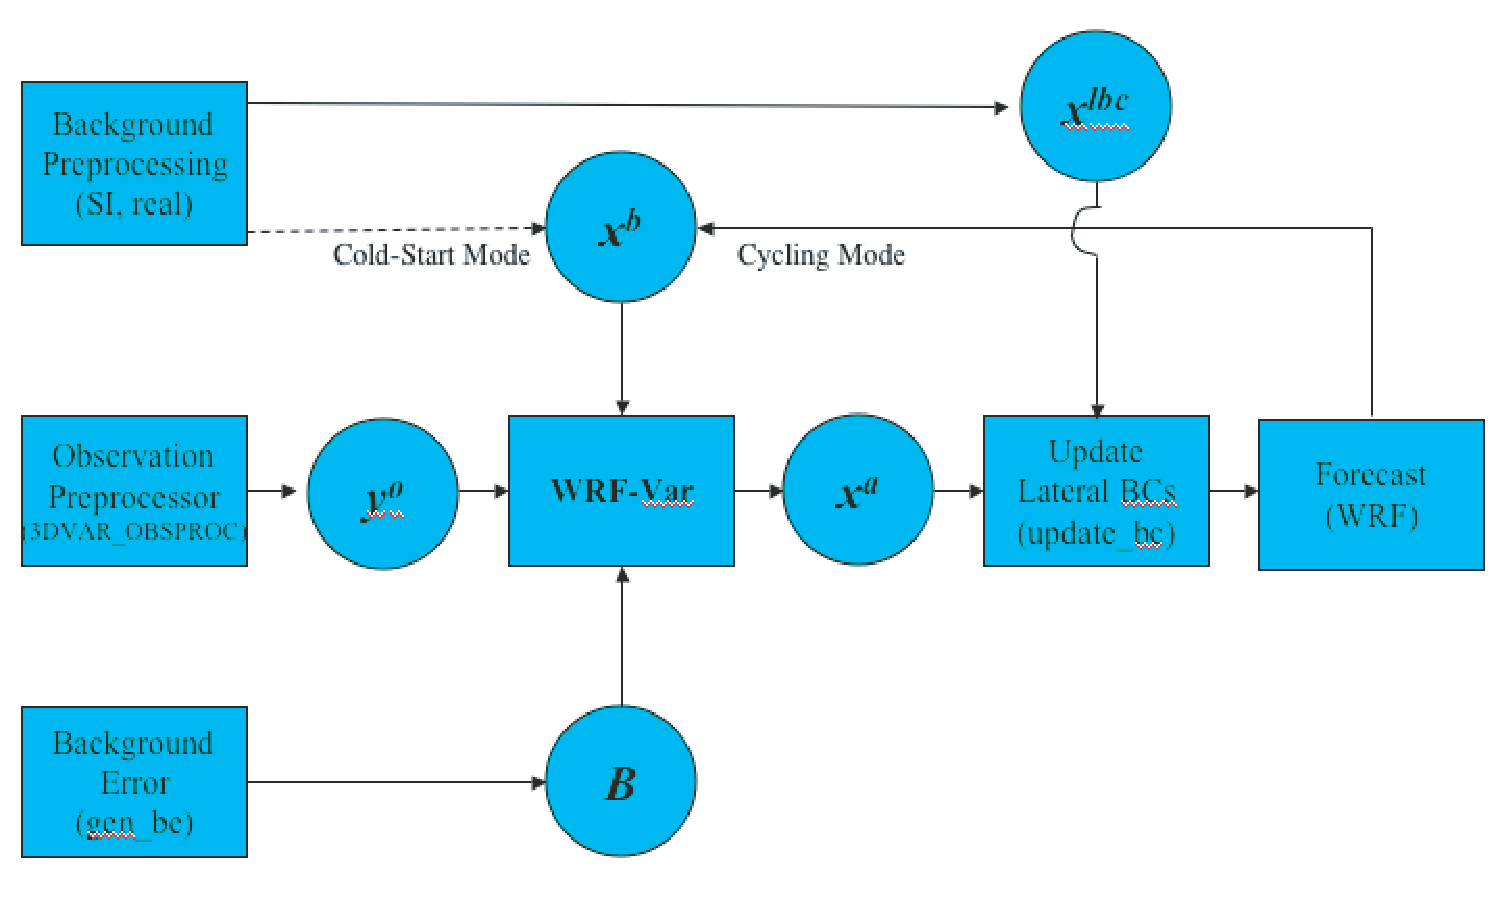
\includegraphics[width=6.5in]{figures/var-sketch.pdf}
  \caption{\label{var-sketch}Sketch showing the relationship between datasets (circles), 
           and algorithms (rectangles) of the ARW system.}
\end{figure}

The three inputs to WRF-Var are: 

\vspace{0.5cm}

a) First guess ${\bf x^{b}}$--- In cold-start mode, this is typically a
forecast/analysis from another model interpolated to the ARW grid (and variables) via the 
WRF SI and {\it real} programs. In cycling mode, the first guess 
is a short-range (typically 1--6 hour) ARW forecast. 

\vspace{0.5cm}

b) Observations ${\bf y^{o}}$--- In the current version of WRF-Var, observations may be 
supplied either in a text (MM5 3D-Var) format or BUFR format (but not a 
combination of the two). An observation preprocessor (3DVAR$\_$OBSPROC) 
is supplied with the code release to perform basic quality control, assign 
observation errors, and reformat observations from the MM5 {\it little$\_$r} text 
format into 3D-Var's own text format. Details can be found in \citet{barker03, barker04}.

\vspace{0.5cm}

c) Background error covariances ${\bf B}$--- used to define the spatial
and multivariate response of the analysis to an observation. In
variational systems, these covariances are typically calculated
off-line, and significant tuning is required to optimize performance
for a particular application (e.g., \citet{ingleby01, wu02}). The
amount of work required to do this satisfactorily is significant, and
should not be underestimated. In order to assist the user, WRF
developers supply the following: i) a default set of statistics used
for the initial set up of a domain; ii) a utility {\it gen$\_$be}
(described in Section
\ref{var-be}) to process ensembles of forecasts into the appropriate control variable 
space; and iii) diagnostic routines to assess the accuracy of
observation and background error statistics. These routines include
both innovation vector-based approaches \citep{hollingsworth86} and
variational tuning approaches \citep{desroziers01}.

Following assimilation of all data, an analysis ${\bf x^{a}}$ is produced that must be 
merged with the existing lateral boundary conditions ${\bf x^{lbc}}$ (described in 
\citet{barker03}). Note: In cycling mode, only the {\it wrfbdy} lateral boundary condition 
files (${\bf x^{lbc}}$) output of SI/real are used, and not the {\it wrfinput} initial condition 
files (${\bf x^{b}}$). In cold-start mode, both are required.

\section{Improvements to the WRF-Var Algorithm}
\label{var-upgrade}

\subsection{Improved vertical interpolation}

The original WRF 3D-Var system described in \citet{barker04} used height 
interpolation for all observation operators. If an observation is reported as a 
function of pressure, then height is approximated using the 
hydrostatic relation. This step introduces an unnecessary source of error. 
The new WRF-Var system performs vertical interpolation in terms of the 
original observed coordinate, i.e., pressure or height.

\subsection{Improved minimization and ``outer loop"}

The default WRF-Var cost function minimization uses a modified version of the limited 
memory Quasi-Newton Method (QNM). Recently, an alternative Conjugate Gradient 
Method (CGM) has been implemented. Unlike the QNM technique, the CGM method 
restricts 3D-Var's inner loop to be completely linear. This limitation is dealt with through 
the inclusion of an outer loop in WRF-Var, the purpose of which is to iterate towards 
nonlinear solutions (e.g., observation operators, balance constraints, and the forecast itself in 
4D-Var) using the WRF-Var analysis from the previous iteration as new background. The 
outer loop is also used as a form of variational quality control as follows: observations are 
rejected if their O-B values are outside a prescribed range (typically several times the 
observation error standard deviation). This {\it errormax} test implicitly assumes the rejected 
large O-B values are due to a bad observation (O) rather than poor background (B). 
However, if it is the background B that is incorrect then the system will reject the most 
useful observations available to the assimilation system, i.e., those in areas where the 
first-guess is poor. The outer loop alleviates this effect by allowing observations 
rejected in previous iterations to be accepted if their new O-B falls within the required range 
in subsequent outer loops. The assimilation of nearby observations in previous iterations 
essentially provides a ``buddy check" to the observation in question.
 
\subsection{Flexible choice of control variables}
\label{var-cvs}

In practical variational data assimilation schemes, the background error covariance 
matrix ${\bf B}$ is computed not in model space ${\bf x}': u, v, T, q, p_{s}$, but in a 
control variable space ${\bf v}$ related to model space via the control variable transform ${\rm U}$, 
i.e.,

\begin{equation}
{\bf x}' = {\rm U}{\bf v}= {\rm U}_{p} {\rm U}_{v} {\rm U}_{h}{\bf v}.
\label{var-cv}
\end{equation}

The expansion ${\rm U}={\rm U}_{p} 
{\rm U}_{v} {\rm U}_{h}$ represents the various stages of covariance modeling: horizontal correlations ${\rm U}_{h}$, vertical covariances ${\rm U}_{v}$, and multivariate covariances
${\rm U}_{p}$.

The components of ${\bf v}$ are chosen so that their error cross-correlations are negligible, 
thus permitting the matrix ${\bf B}$ to be block-diagonalized. The many varying applications 
(high/low resolution, polar/tropical, etc.) of WRF-Var require a flexible 
choice of background error model. This is achieved via a namelist option 
``cv$\_$options" as defined in Table \ref{var-cvtable}.

\begin{table}[h]
\begin{center}
\begin{tabular}{|l|l|l|l|l|l|}
\hline
% Line 1
 { } &
 \ &
 \multicolumn{1}{c|}{2} &
 \multicolumn{1}{c|}{3} & 
 \multicolumn{1}{c|}{4} &
 \multicolumn{1}{c|}{5} \\
 \raisebox{1.5ex}[0cm] {cv$\_$options} & 
 \ &
 \multicolumn{1}{c|}{(original MM5)} &
 \multicolumn{1}{c|}{(NCEP)} &
 \multicolumn{1}{c|}{(Global)} &
 \multicolumn{1}{c|}{(Regional)}\\
 \hline
% Line 2
 { } &
 \multicolumn{1}{c|}{ } &
 \multicolumn{4}{c|}{ }\\
 \raisebox{1.5ex}[0cm] {Analysis} & 
 \multicolumn{1}{c|}{${\bf x}'$} &
 \multicolumn{4}{c|}{$u'$,$v'$,$T'$,$q'$,${p_s}'(i,j,k)$}\\
 \raisebox{1.5ex}[0cm] {Increment} & 
 \multicolumn{1}{c|}{ } &
 \multicolumn{4}{c|}{ }\\
 \hline
% Line 3
 { } &
 \multicolumn{1}{c|}{ } &
 \multicolumn{1}{c|}{ } &
 \multicolumn{3}{c|}{ }\\
 \raisebox{1.5ex}[0cm] {Change of} & 
 \multicolumn{1}{c|}{${\rm U}_p$} &
 \multicolumn{1}{c|}{$\psi'$,$\chi'$,$p_u'$,$q'$} &
 \multicolumn{3}{c|}{$\psi'$,$\chi_u'$,$T_u'$,$r'$,$p_{su}'$}\\
 \raisebox{1.5ex}[0cm] {Variable} & 
 \multicolumn{1}{c|}{ } &
 \multicolumn{1}{c|}{ } &
 \multicolumn{3}{c|}{ }\\
 \hline
% Line 4
 { } &
 \multicolumn{1}{c|}{ } &
 \multicolumn{1}{c|}{ } &
 \multicolumn{1}{c|}{ } &
 \multicolumn{2}{c|}{ }\\
 \raisebox{1.5ex}[0cm] {Vertical} &
 \multicolumn{1}{c|}{${\rm U}_v$} &
 \multicolumn{1}{c|}{${\bf B}={\bf E}{\Lambda}{\bf E}^{T}$} &
 \multicolumn{1}{c|}{RF} &
 \multicolumn{2}{c|}{${\bf B}={\bf E}{\Lambda}{\bf E}^{T}$} \\
 \raisebox{1.5ex}[0cm] {Covariances} &
 \multicolumn{1}{c|}{ } &
 \multicolumn{1}{c|}{ } &
 \multicolumn{1}{c|}{ } &
 \multicolumn{2}{c|}{ }\\
 \hline
% Line 5
 { } &
 \multicolumn{1}{c|}{ } &
 \multicolumn{2}{c|}{ } &
 \multicolumn{1}{c|}{ } &
 \multicolumn{1}{c|}{ }\\
 \raisebox{1.5ex}[0cm] {Horizontal} &
 \multicolumn{1}{c|}{${\rm U}_h$} &
 \multicolumn{2}{c|}{RF} &
 \multicolumn{1}{c|}{Spectral} &
 \multicolumn{1}{c|}{RF}\\
 \raisebox{1.5ex}[0cm] {Correlations} &
 \multicolumn{1}{c|}{ } &
 \multicolumn{2}{c|}{ } &
 \multicolumn{1}{c|}{ } &
 \multicolumn{1}{c|}{ }\\
 \hline
% Line 6
 { } &
 \multicolumn{1}{c|}{ } &
 \multicolumn{2}{c|}{ } &
 \multicolumn{1}{c|}{ } &
 \multicolumn{1}{c|}{ }\\
 \raisebox{1.5ex}[0cm] {Control} &
 \multicolumn{1}{c|}{${\bf v}$ } &
 \multicolumn{1}{c|}{${\bf v}(i,j,m)$} &
 \multicolumn{1}{c|}{${\bf v}(i,j,k)$} &
 \multicolumn{1}{c|}{${\bf v}(l,n,m)$} &
 \multicolumn{1}{c|}{${\bf v}(i,j,m)$}\\
 \raisebox{1.5ex}[0cm] {Variables} &
 \multicolumn{1}{c|}{ } &
 \multicolumn{2}{c|}{ } &
 \multicolumn{1}{c|}{ } &
 \multicolumn{1}{c|}{ }\\
 \hline
\end{tabular}
\end{center}
\caption{The definitions of the various stages of the control
     variable transform given by (\ref{var-cv}) for the unified global/regional
     WRF-Var system. Indices $(i,j,k)$ refer to grid-point
     space, index $m$ to vertical mode, and $l$, $n$ to global spectral mode.
     The variables are: $u, v$: velocity components; $T$: temperature; $q$: mixing ratio;
     $p_s$: surface pressure; $\psi$: streamfunction; $\chi$: velocity potential;
     $r$: relative humidity. The subscript $u$ indicates an unbalanced field. The acronym RF stands for recursive filter.}
\label{var-cvtable}
\end{table}

Table \ref{var-cvtable} indicates that the only difference between global (cv$\_$options=4) and WRF 
regional (cv$\_$options=5) versions of the WRF-Var control variable 
transform is in the horizontal error correlations ${\rm U}_{h}$. 
Note also, the only difference between the old MM5 
background error model (cv$\_$options=2) and WRF regional (cv$\_$options=5) is in the 
${\rm U}_{p}$ transform. The former imposes a dynamical balance constraint via an 
unbalanced pressure control variable \citep{barker04}, whereas in the new regional 
covariance model, balance is imposed via statistical regression (see Section \ref{var-be} for 
details). This choice of control variables is considered more appropriate for the 
mass-based ARW solver.

\subsection{First Guess at Appropriate Time (FGAT)}

A First Guess at Appropriate Time (FGAT) procedure has been implemented in 
WRF-Var \citep{lee04}.
 The FGAT capability results in a more accurate calculation of innovation vectors 
(observation minus first guess difference), and hence a better use of observations when 
their valid time differs from that of the analysis. 
FGAT is most effective for the analysis of observations from 
asynoptic, moving platforms (e.g., aircraft and satellite data). Surface observations with 
high temporal resolution also benefit from the use of FGAT.

\subsection{Radar Data Assimilation}

Numerous modifications have been made in order to assimilate Doppler
radar radial velocity and reflectivity observations. Firstly, vertical
velocity increments are included in WRF-Var via the ``Richarson
balance equation" that combines the continuity equation, adiabatic
thermodynamic equation, and hydrostatic relation. Linear and adjoint
codes of Richardson's equation have been incorporated into WRF-Var. In
order to develop a capability for Doppler reflectivity assimilation,
we use the total water as a control variable, requiring a partitioning
of the moisture and water hydrometeor increments. A warm-rain
parameterization is also included, which includes condensation of
water vapor into cloud, accretion of cloud by rain, automatic
conversion of cloud to rain, and evaporation of rain to water
vapor. Finally, the observation operators for Doppler radial velocity
and reflectivity are included in WRF-Var. Further details and results
of the radial velocity work can be found in \citet{xiao05}. The radar
reflectivity approach will be described in a future paper.

\subsection{Unified Regional/Global 3D-Var Assimilation}

There are many benefits to having a single data assimilation system
for regional and global applications. The majority of the code is
common to both (observation operators, minimization, background error
preconditioning, interpolation, etc.). Technically, the main changes
required to extend the regional application to global are related to
the presence of a) the polar singularity, and b) periodic East-West
boundary conditions. Of course, there are also scientific questions
concerning the optimal mix of observations required for
global/regional models, and the choice of control variables and
balance constraints. A unified global/regional 3D-Var system should
therefore be flexible to a variety of thinning/quality-control
algorithms and also to alternative formulations of the background
error covariance matrix. This flexibility has been a key design
requirement throughout the WRF-Var project.

The major difference between regional and global options in WRF-Var is
in the definition of horizontal background error covariances. In
regional mode, recursive filters \citep{purser03} are used to project
observation information away from the observation location. In global
mode, a spectral decomposition is applied. The main benefits of the
spectral technique are a) the isotropic and homogeneous covariances
that are implied neatly solve the problems associated with the pole
(the pole is not a special point in spectral space), and b) horizontal
correlations are defined in terms of a single function--- the power
spectrum (a function of total wavenumber). However, the isotropy of
correlation defined in spectral space is also a weakness---
anisotropies need to be defined in an alternative manner. One solution
to this problem is to replace the spectral correlations with
grid-point correlations (e.g., in the Gridpoint Statistical
Interpolation scheme under development at NCEP). An alternative
technique is to supplement the isotropic spectral correlations with an
anisotropic component derived via grid transformations, additional
control variables or 4D-Var. Research using the latter techniques is
underway using the WRF-Var system.

The WRF-Var code has been adapted to perform assimilation on a global, regular 
latitude-longitude grid. The major modifications are as follows.

\vspace{0.5cm}

a) Spectral to grid-point transformations (and their adjoints) have been included in 3D-Var 
to represent the horizontal component (${\rm U}_h$) of the background error covariance 
model.

\vspace{0.5cm}

b) A new global WRF-Var registry was created to accommodate the 
output of global forecast models (currently only the Korean Meteorological 
Administration's (KMA) global model has been tested). 
The final analysis increments are written in binary format and added back to the global 
first guess to provide the global analysis in the native model format.

\vspace{0.5cm}

c) Changes have been made to allow for periodic boundary conditions in the East--West 
direction.

\vspace{0.5cm}

d) A number of minor changes have been made to treat the polar rows as special points 
(e.g., in the grid-point $\psi, \chi$ to $u,v$ wind conversion in the ${\rm U}_p$ transform and the 
observation operators for polar winds).

\section{Background Error Covariances}
\label{var-be}

Forecast (``first guess" or ``background") error covariances are a vital input to variational 
data assimilation systems. They influence the analysis fit to observations and also 
completely define the analysis response away from observations. The latter impact is 
particularly important in data-sparse areas of the globe. Unlike ensemble filter data 
assimilation techniques (e.g., the Ensemble Adjustment Kalman Filter, the Ensemble 
Transform Kalman Filter), 3/4D-Var systems do not implicitly evolve forecast error 
covariances in real-time. Instead, climatologic statistics are usually estimated offline. 
The ``NMC-method", in which forecast error covariances are approximated using 
forecast difference (e.g., T+48 minus T+24) statistics, is a commonly used approach 
\citep{parrish92}. Experiments at ECMWF \citep{fisher03} indicate superior statistics may 
be obtained using a cycling analysis/forecast ensemble prediction
system based on perturbed observations/physics.

Recent advances permit the use of flow-dependent forecast error
covariances in 3D/4D-Var through, for example, grid transformations
\citep{desroziers97}, anisotropic recursive filters
\citep{wu02, purser03},
or observation-space formulations of the variational 
problem \citep{daley01}. Flow-dependence may be enhanced in 4D-Var 
through the use of the forecast model to provide dynamical consistency to the evolving 
forecast state during 4D-Var's time window \citep{rabier98}. Still, the practical effort 
required to specify and implement flow-dependent error covariances in 3/4D-Var is 
significant.

The NMC-method code developed for MM5 3D-Var \citep{barker04} is nearing the 
end of its useful life. The development of a unified global/regional WRF-Var system, and 
its application to a variety of models (e.g., ARW, MM5, KMA global model, 
Taiwan's Nonhydrostatic Forecast System [NFS]) has 
required a new, efficient, portable forecast background error covariance calculation 
code to be written. There is also a demand for such a capability to be available and 
supported for the wider 3/4D-Var research community for application to their own 
geographic areas of interest (the default statistics supplied with the WRF-Var 
release are designed only as a starting point). In this section, the new {\it gen$\_$be} code 
developed by NCAR/MMM to generate forecast error statistics for use with the 
WRF-Var system is described.

The background error covariance matrix is defined as 

\begin{equation}
{\bf B}=\overline{\epsilon \epsilon^{T}} \simeq \overline{{\bf x'}{\bf x'}^{T}},
\label{var-b}
\end{equation}

\noindent where the overbar denotes an average over time and/or geographical area. The true 
background error $\epsilon$ is not known in reality, but is assumed to be statistically
well-represented by a model state perturbation ${\bf x'}$. In the standard NMC-method
\citep{parrish92}, the perturbation ${\bf x'}$ is given by the difference between 
two forecasts (e.g., 24 hour minus 12 hour) verifying at the same time. Climatological 
estimates of background error may then be obtained by averaging such forecast 
differences over a period of time (e.g., one month). An alternative strategy proposed by 
\citep{fisher03} makes use of ensemble forecast output, defining the ${\bf x'}$ vectors as 
ensemble perturbations (ensemble minus ensemble mean). In either approach, the end 
result is an ensemble of model perturbation vectors from which estimates of 
background error may be derived. The new {\it gen$\_$be} utility has been designed to work with 
either forecast difference, or ensemble-based, perturbations.

As described above, the WRF-Var background error covariances are specified not in 
model space ${\bf x'}$, but in a control variable space ${\bf v}$, which is related to the model variables 
(e.g., wind components, temperature, humidity, and surface pressure) via the control 
variable transform defined in (\ref{var-cv}). Both (\ref{var-cv}) and 
its adjoint are required in WRF-Var. In contrast, the background error code performs the 
inverse control variable transform ${\bf v}={\rm U}_{h}^{-1} {\rm U}_{v}^{-1} {\rm U}_{p}^{-1}{\bf x'}$ in order to 
accumulate statistics for each component of the control vector ${\bf v}$.

Using the NMC-method, ${\bf x}'={\bf x_{T2}}-{\bf x_{T1}}$ where $T2$ and $T1$ 
are the forecast difference times (e.g., 48h minus 24h for global, 24h minus 12h for regional). 
Alternatively, for an ensemble-based approach, ${\bf x_{k}}'={\bf x_{k}}-\bar{\bf 
x}$, where the overbar is an average over ensemble members $k=1,n_{e}$. The total 
number of binary files produced by this stage is $n_{f} \times n_e$ where $n_f$ is the 
number of forecast times used (e.g., for 30 days with forecast every 12 hours, $n_f=60$). 
Using the NMC-method, $n_e=1$ (1 forecast difference per time). For ensemble-based 
statistics, $n_e$ is the number of ensemble members.

The background error covariance generation code {\it gen$\_$be} is designed to process
data from a variety of regional/global models (e.g., ARW, MM5, KMA global model, 
NFS, etc.), and process it in order to provide error 
covariance statistics for use in variational data assimilation systems. The initial, 
model-dependent ``stage 0" is illustrated in Fig. \ref{var-genbe0}. 

%
%   Figure 9.6 var-genbe0
%
\begin{figure}
  \centering
  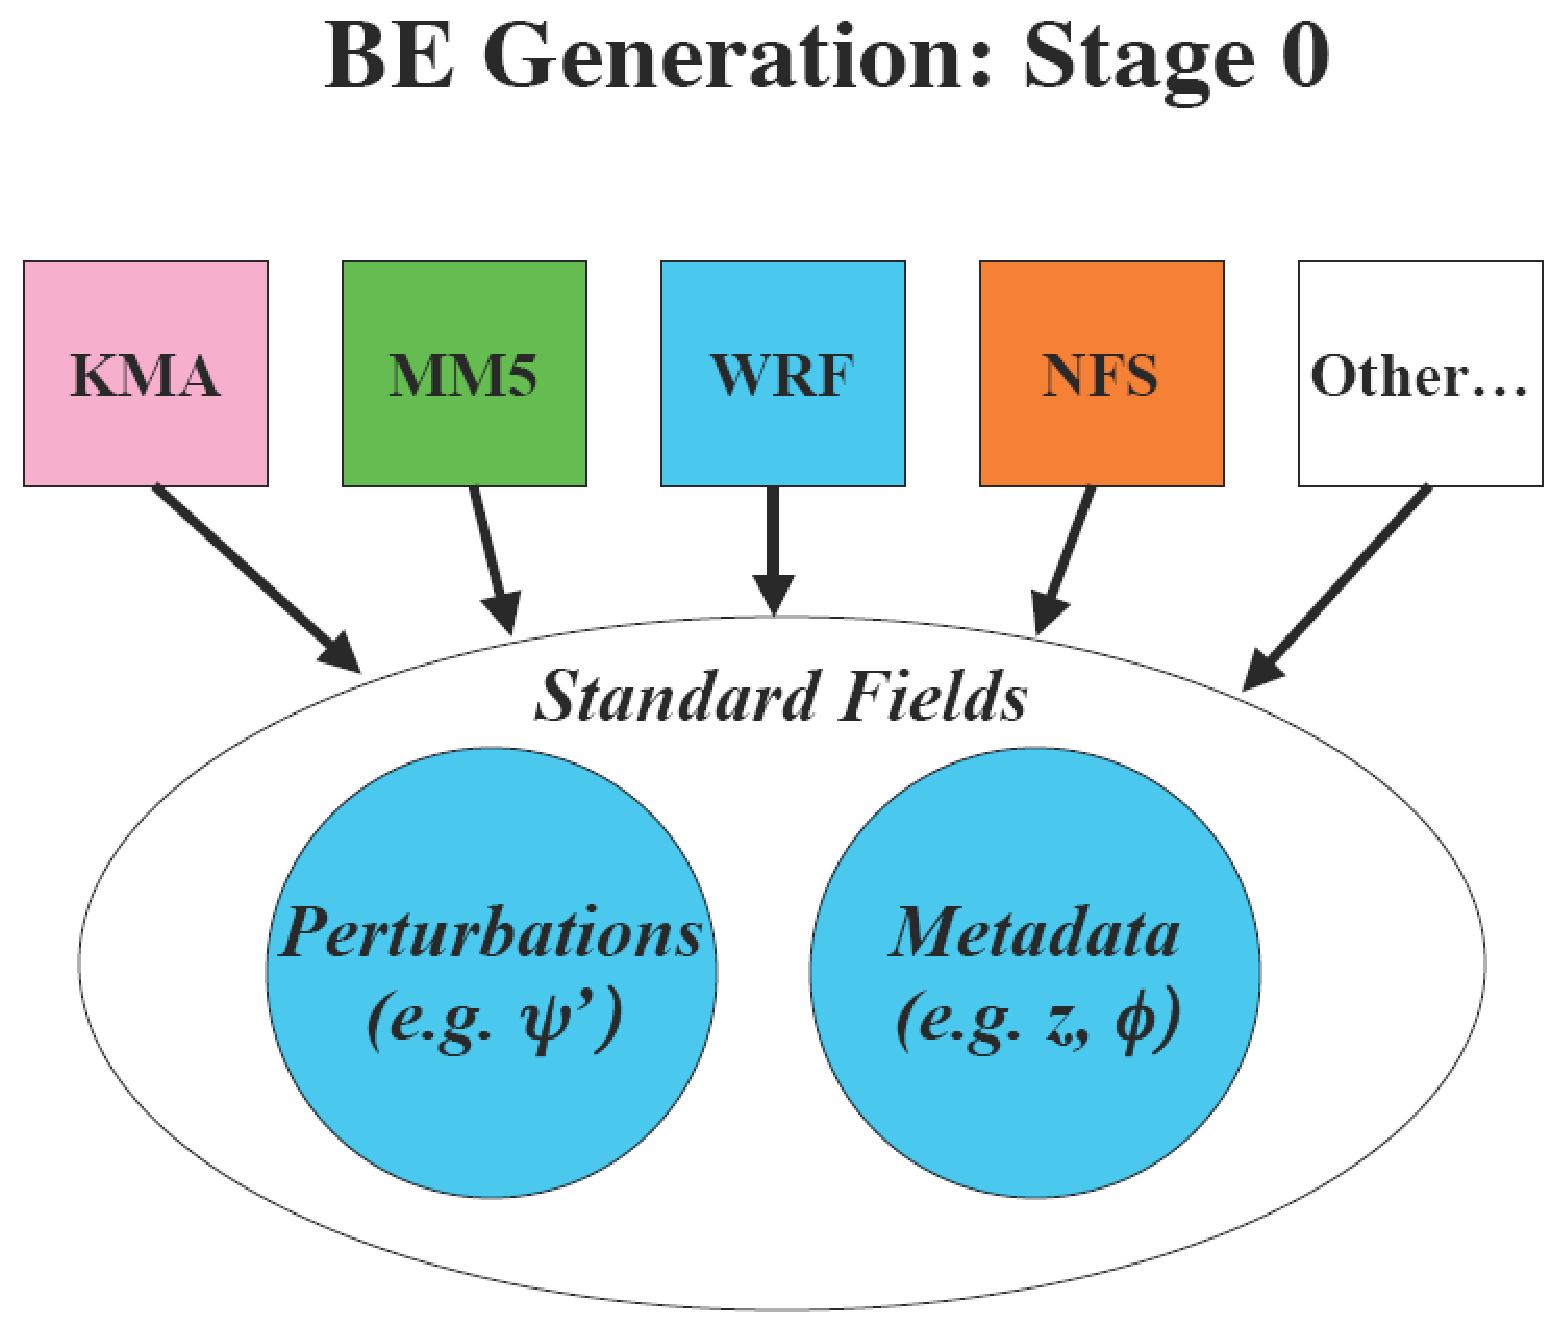
\includegraphics[width=4.0in]{figures/var-genbe0.pdf}
  \caption{\label{var-genbe0}Sketch of the role of Stage 0 converters 
  in transforming model-specific data (e.g., ARW, KMA global model, etc.) to standard 
  perturbation fields and relevant metadata (e.g., latitude, height, land/sea, etc.).}
\end{figure}

Alternative models use different grids, variables, data formats, etc., and so initial converters 
are required to transform model output into a set of standard perturbation fields (and metadata), 
and to output them in a standard binary format for further, model-independent processing. The 
standard grid-point fields are as follows.

\begin{itemize}\setlength{\parskip}{-4pt}
\item
 	Perturbations: Streamfunction $\psi'(i,j,k)$, velocity potential $\chi'(i,j,k)$, 
temperature $T'(i,j,k)$, relative humidity $r'(i,j,k)$, surface pressure $p_s'(i,j)$.

\item
 	Full-fields: height $z(i,j,k)$, latitude $\phi(i,j)$. (These are required for the 
production of background error statistics stored in terms of physics variables, 
rather than tied to a specific grid. This flexibility is included in {\it gen$\_$be} through a 
namelist option to define the bins over which data is averaged in a variety of ways 
(e.g., latitude height, grid points). Land-sea and orographic effects may also be 
represented in this way.
\end{itemize}

In general, the {\it stage$\_$0} converters are developed and maintained by those supporting
individual models. Only the WRF-to-standard-fields converter {\it gen$\_$be$\_$stage0$\_$wrf} 
is maintained and supported by the ARW effort.

\subsection{Removal of time-mean}

In order to calculate covariances between fields, the average value must first be removed. 
This is performed in the first stage utility {\it gen$\_$be$\_$stage1}. 

\subsection{Multivariate Covariances: Regression coefficients and unbalanced variables}

The WRF-Var system permits a variety of background error covariance
models to be employed, as described in Section \ref{var-cvs}
above. 
The utility {\it gen$\_$be} is used to provide background error
statistics only for cv$\_$options 4 and 5.  

The second stage
of {\it gen$\_$be (gen$\_$be$\_$stage2)} provides statistics for the
unbalanced fields $\chi_u$, $T_u$, and $P_{su}$ used as control
variables in WRF-Var. The unbalanced control variables are defined as
the difference between full and balanced (or correlated) components of
the field. In this stage of the calculation of background errors, the
balanced component of particular fields is modeled via a regression
analysis of the field using specified predictor fields
(e.g., streamfunction; see
\citet{wu02} for further details). The resulting regression coefficients 
are output for use 
in WRF-Var's ${\rm U}_p$ transform. Currently, three regression analyses are
performed resulting in three sets of regression coefficients (Note:
The perturbation notation has been dropped for the 
remainder of this chapter for clarity.):

\begin{itemize}\setlength{\parskip}{-4pt}
\item   Velocity potential/streamfunction regression: $\chi_b=c\psi$;
\item	Temperature/streamfunction regression: $T_{b,k1}=\sum_{k2}G_{k1,k2}\psi_{k2}$; and
\item	Surface pressure/streamfunction regression: $p_{sb}=\sum{k}W_{k}\psi_{k}$.
\end{itemize}

Data is read from all $n_f \times n_e$ files and sorted into bins defined via the namelist 
option {\it bin$\_$type}. Regression coefficients $G(k1,k2)$ and $W(k)$ are computed 
individually for each bin (bin$\_$type=1 is used here, representing latitudinal dependence) 
in order to allow representation of differences between, for example, polar, mid-latitude, and 
tropical dynamical and physical processes. In addition, the scalar coefficient $c$ used to 
estimate velocity potential errors from those of streamfunction is calculated as a function 
of height to represent, for example, the impact of boundary-layer physics. Latitudinal/height 
smoothing of the resulting coefficients may be optionally performed to avoid artificial 
discontinuities at the edges of latitude/height boxes.

Having computed regression coefficients, the unbalanced components of the fields are 
calculated as $\chi_u=\chi-c\psi$, $T_{u,k1}=T_{k1}-\sum_{k2}G_{k1,k2}\psi_{k2}$, 
and $p_{su}=p_s - \sum_{k} W_{k}\psi_{k}$. These fields are output for the 
subsequent calculation of the spatial covariances as described below.

\subsection{Vertical Covariances: Eigenvectors/eigenvalues and 
control variable projections}

The third stage ({\it gen$\_$be$\_$stage3}) of {\it gen$\_$be}
calculates the statistics required for the vertical component of the
control variable transform. This calculation involves the projection
of 3D fields on model-levels onto empirical orthogonal functions
(EOFs) of the vertical component of background error covariances
\citep{barker04}. For each 3D control variable ($\psi$, $\chi_u$,
$T_u$, and $r$), the vertical component of ${\bf B}$, is calculated
and an eigenvector decomposition performed. The resulting eigenvectors
${\bf E}$ and eigenvalues $\Lambda$ are saved for use in WRF-Var.

The {\it gen$\_$be} code calculates both domain-averaged and local
values of the vertical component of the background error covariance
matrix. The definition of local again depends on the value of the
namelist variable bin$\_$type chosen. For example, for bin$\_$type=1,
a $kz \times kz$ (where $kz$ is the number of vertical levels) vertical
component of $\bf B$ is produced at every latitude (data is averaged
over time and longitude) for each control variable. Eigendecomposition
of the resulting climatological vertical error covariances ${\bf
B}={\bf E}{\Lambda}{\bf E}^{T}$ results in both domain-averaged and
local eigenvectors $\bf E$ and eigenvalues $\Lambda$. Both sets of
statistics are included in the dataset supplied to WRF-Var, allowing
the choice between homogeneous (domain-averaged) or local
(inhomogeneous) background error variances and vertical correlations
to be chosen at run time \citep{barker04}.
Having calculated and stored eigenvectors and eigenvalues, the final
part of {\it gen$\_$be$\_$stage3} is to project the entire sequence of
3D control variable fields into EOF space ${\bf v_v}=U_{v}^{-1}{\bf
v_p}=\Lambda^{-1/2}{\bf E}^{T} {\bf v_p}$.

\subsection{Horizontal Covariances: Recursive filter lengthscale (regional), or power 
spectra (global)}

The last aspect of the climatological component of background error
covariance data required for WRF-Var is the horizontal error
correlations, the representation of which forms the largest difference
between running WRF-Var in regional and global mode. (It is however,
still a fairly local change.)

In a global application ({\it gen\_be\_stage4\_global}), power spectra
are computed for each of the $kz$ vertical modes of the 3D control
variables $\psi$, $\chi_u$, $T_u$, and $r$, and for the 2D control
variable $p_{su}$ data. In contrast, in regional mode, horizontal
correlations are computed between grid-points of each 2D field, binned
as a function of distance. A Gaussian curve is then fitted to the data
as described in \citet{barker04} to provide correlation lengthscales
for use in the recursive filter algorithm.

